\begin{figure}[h]
\centering
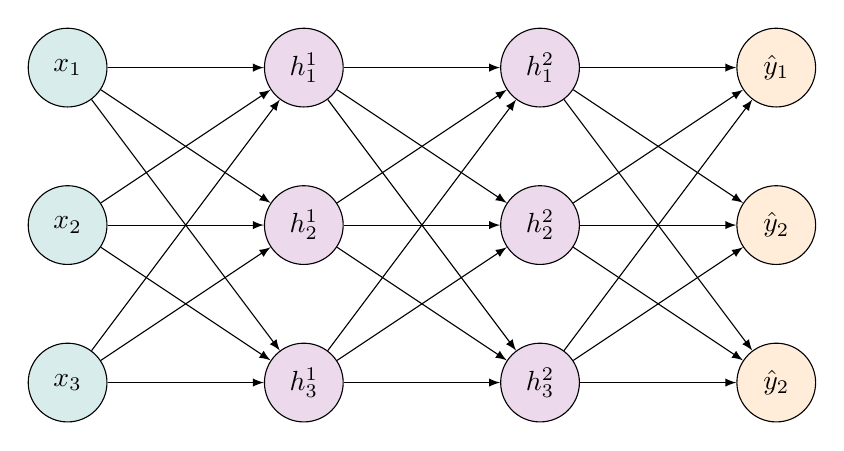
\begin{tikzpicture}[
    neuron/.style={circle, draw, minimum size=1cm, align=center},
    input/.style={neuron, fill=teal!15},
    hidden/.style={neuron, fill=violet!15},
    output/.style={neuron, fill=orange!15},
    arrow/.style={-latex, thick}
]

% Input layer neurons
\node[input]  (x1) at (0,  2)  {$x_1$};
\node[input]  (x2) at (0,  0)  {$x_2$};
\node[input]  (x3) at (0, -2)  {$x_3$};

% Hidden layer 1 neurons
\node[hidden] (h11) at (3,  2)  {$h_1^1$};
\node[hidden] (h12) at (3,  0)  {$h_2^1$};
\node[hidden] (h13) at (3, -2)  {$h_3^1$};

% Hidden layer 2 neurons
\node[hidden] (h21) at (6,  2)  {$h_1^2$};
\node[hidden] (h22) at (6,  0)  {$h_2^2$};
\node[hidden] (h23) at (6, -2)  {$h_3^2$};

% Output layer neurons
\node[output] (y1) at (9,  2)  {$\hat{y}_1$};
\node[output] (y2) at (9, 0)  {$\hat{y}_2$};
\node[output] (y3) at (9, -2)  {$\hat{y}_2$};

% Input to hidden layer 1 connections
\foreach \i in {1,2,3}{
    \foreach \j in {1,2,3}{
        \draw[-latex] (x\i) -- (h1\j);
    }
}

% Hidden layer 1 to hidden layer 2 connections
\foreach \i in {1,2,3}{
    \foreach \j in {1,2,3}{
        \draw[-latex] (h1\i) -- (h2\j);
    }
}

% Hidden layer 2 to output connections
\foreach \i in {1,2,3}{
    \foreach \j in {1,2,3}{
        \draw[-latex] (h2\i) -- (y\j);
    }
}

% Layer labels
% \node at (0,  -3.2) {\small Input layer};
% \node at (3,  -3.2) {\small Hidden layer 1};
% \node at (6,  -3.2) {\small Hidden layer 2};
% \node at (9,  -3.2) {\small Output layer};

\end{tikzpicture}
\caption{A Multilayer Perceptron.}
\label{fig:mlp}
\end{figure}
